\section{Preliminary: On-Policy Distillation}

\begin{figure}[t]
    \centering
    \begin{subfigure}[c]{0.5\textwidth}
        \centering
        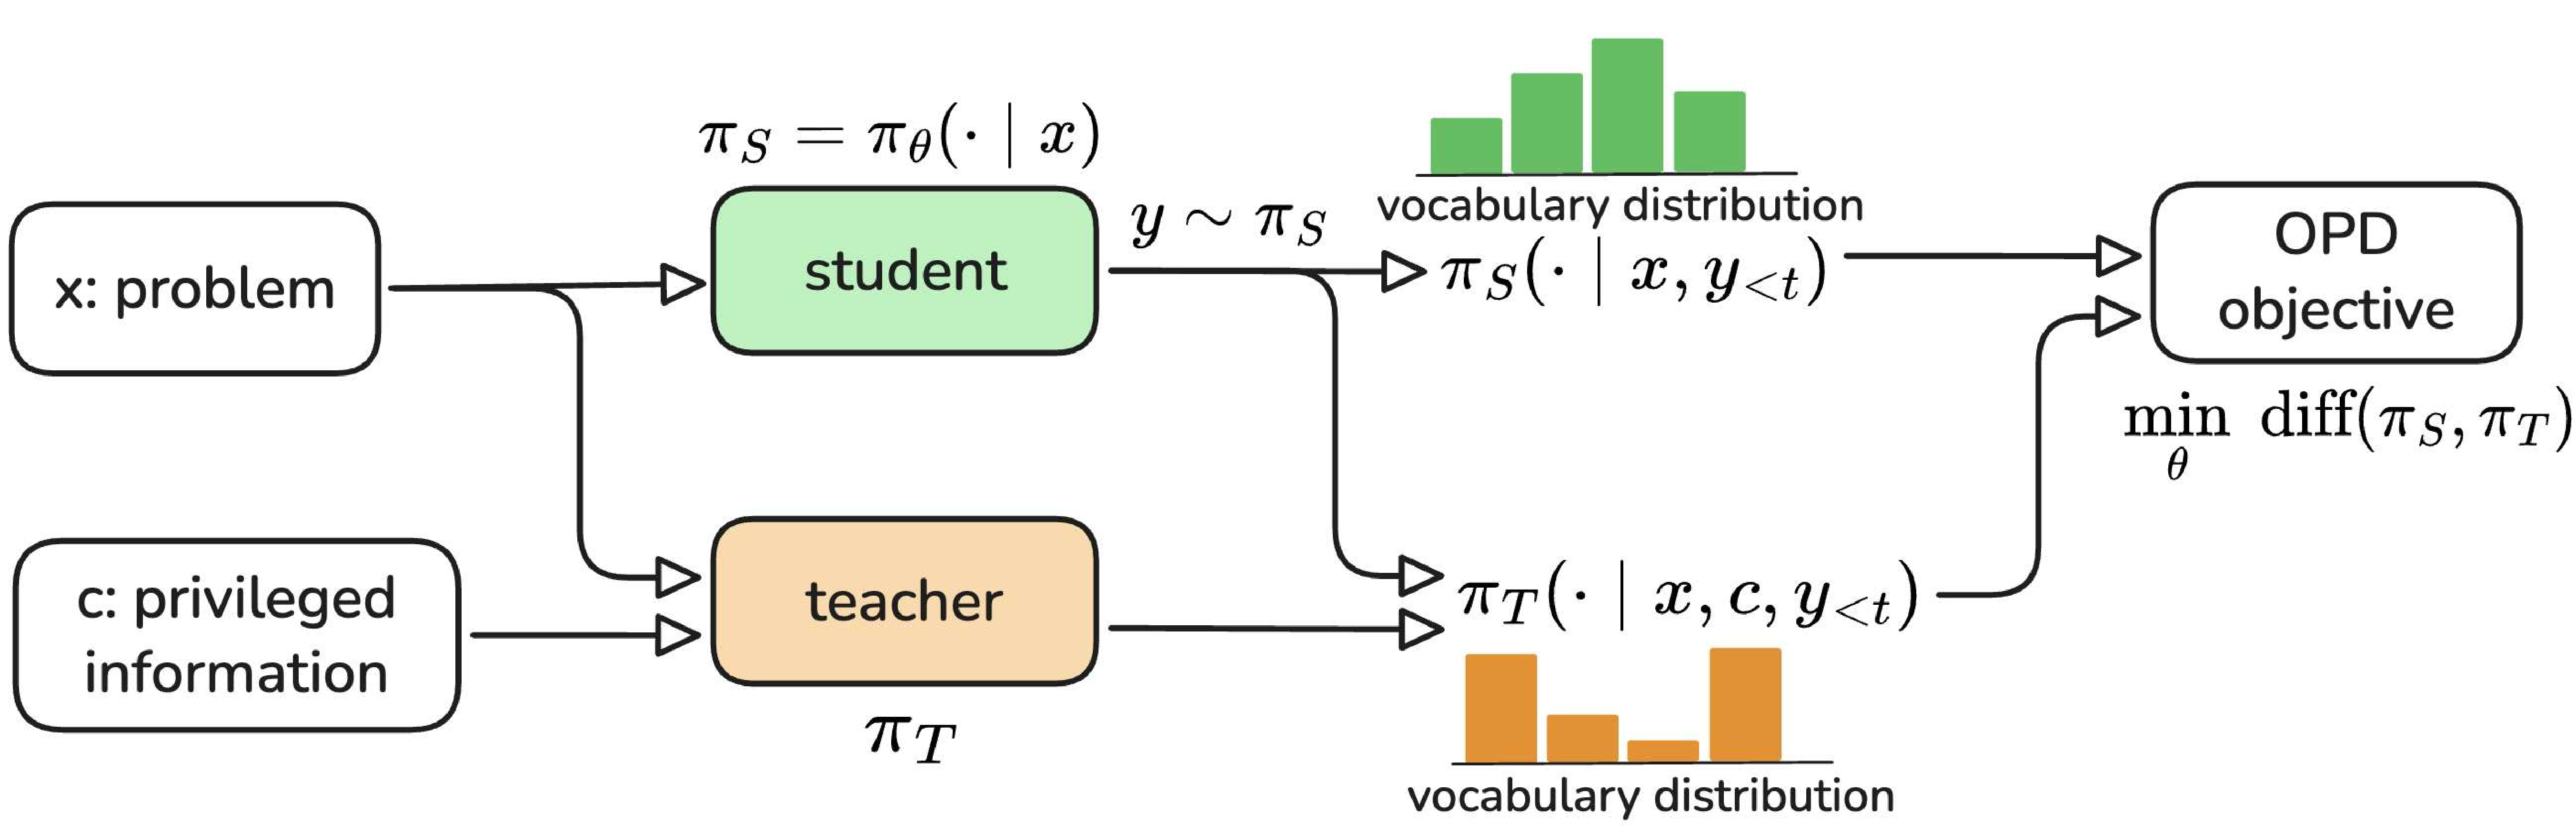
\includegraphics[width=\textwidth]{figures/opsdfig1.pdf}
        \label{fig:first}
    \end{subfigure}
    \begin{subfigure}[c]{0.23\textwidth}
        \centering
        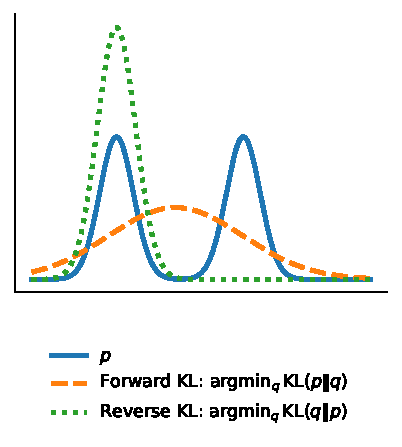
\includegraphics[width=\textwidth]{figures/reverse_forward_kl_only_4th.pdf}
        \label{fig:second}
    \end{subfigure}
    \vspace{-7mm}
    \caption{(\textbf{Left}) On-Policy (Self-)Distillation. In OPSD, the teacher is constructed from the student itself and privileged information (PI) is necessary. In OPD, the teacher is a stronger model and PI is optional. (\textbf{Right}) \textbf{p}: teacher distribution, \textbf{q}: student distribution. Reverse KL is mode-seeking, whereas forward KL is mode-covering.}
    \label{fig:teaser}
\end{figure}


% \begin{figure}[t]
%     \centering
%     \begin{minipage}[c]{0.52\textwidth}
%         \centering
%         \begin{subfigure}[c]{0.5\textwidth}
%             \centering
%             \includegraphics[width=\textwidth]{figures/opsdfig.pdf}
%             \label{fig:first}
%         \end{subfigure}
%         \hspace{2mm}
%         \begin{subfigure}[c]{0.32\textwidth}
%             \centering
%             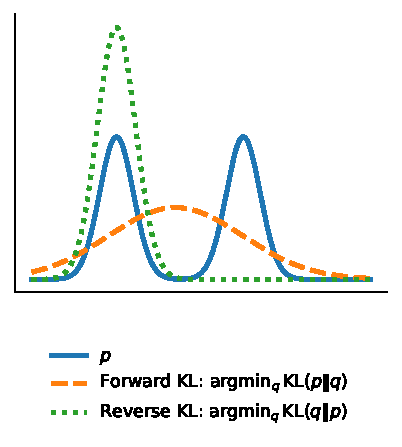
\includegraphics[width=\textwidth]{figures/reverse_forward_kl_only_4th.pdf}
%             \label{fig:second}
%         \end{subfigure}
%     \end{minipage}
%     \hfill
%     \begin{minipage}[c]{0.44\textwidth}
%         \caption{
%         (\textbf{Left}) On-policy (self) distillation with privileged information (PI).
%         In OPSD, the teacher is constructed from the student itself and PI is necessary.
%         In OPD, the teacher is a stronger model and PI is optional.
%         (\textbf{Right}) Reverse KL is mode-seeking, whereas forward KL is mode-covering.
%         }
%         \label{fig:teaser}
%     \end{minipage}
% \end{figure}

Let $x\sim\mathcal D$ be an input, $\pi_\theta$ be the student policy, and
$\pi_T(\cdot\mid x,I)$ be the teacher policy with optional privileged information
$I$. In OPD, $\pi_T$ is a stronger external model. In OPSD, $\pi_T$ is a
student-derived policy augmented with PI.  As illustrated in Figure~\ref{fig:teaser}, OP(S)D trains on student-generated trajectories
$y=(y_1,\ldots,y_T)\sim\pi_\theta(\cdot\mid x)$. At each prefix $y_{<t}$, the
student receives token-level supervision from the teacher:
\begin{equation}
\mathcal L_{\mathrm{OP(S)D}}
=
\mathbb E_{x,y}
\left[
\frac{1}{T}\sum_{t=1}^T
\ell_t\!\left(
\pi_\theta(\cdot\mid x,y_{<t}),
\operatorname{stograd}\!\left(\pi_T(\cdot\mid x,y_{<t},I)\right)
\right)
\right].
\end{equation}

\paragraph{Full-vocabulary KL.}
A standard choice for $\ell_t$ is to match the teacher and student vocabulary with reverse KL:
\begin{equation}
D_{\mathrm{KL}}(\pi_\theta\|\pi_T)
=
\sum_v \pi_\theta(v)\log\frac{\pi_\theta(v)}{\pi_T(v)} .
\label{eq:fullreverseKL}
\end{equation}
Forward KL is mode-covering and encourages the student to cover the teacher
distribution. Reverse KL is mode-seeking and tends to preserve the student's
high-probability modes, making it less prone to catastrophic forgetting \cite{chan2022greedificationoperatorspolicyoptimization}. In OPD, forward KL is undesirable because it pushes the student toward teacher-preferred but student-unlikely tokens. 

For reverse KL, writing $p_\theta(v)=\pi_\theta(v\mid x,y_{<t})$
and $p_T(v)=\pi_T(v\mid x,y_{<t},I)$, its gradient is
\begin{equation}
\nabla_\theta D_{\mathrm{KL}}(p_\theta\|p_T)
=
\sum_v p_\theta(v)
\left[
\log\frac{p_\theta(v)}{p_T(v)} \cancel{\textbf{+1}}
\right]
\nabla_\theta \log p_\theta(v).
\end{equation}
In the full vocabulary, the constant $\textbf{+1}$ has zero contribution since
$
\sum_v p_\theta(v)\nabla_\theta\log p_\theta(v) = 0 .
$


\paragraph{Sampled-token KL.}
Another choice of $\ell_t$ uses the sampled token $y_t\sim\pi_\theta$.
The sampled-token objective treats the teacher-student log-probability gap as an advantage:
\begin{equation}
\mathcal L_{\mathrm{PG}}
=
-\mathbb E_{y\sim\pi_\theta}
\sum_t
\textbf{stopgrad}\big(\log\pi_T(y_t\mid x,y_{<t},I)
-\log\pi_\theta(y_t\mid x,y_{<t})\big)
\log\pi_\theta(y_t\mid x,y_{<t}),
\label{eq:policygrad_sampledtoken}
\end{equation}
whose policy-gradient form is
\begin{equation}
\nabla_\theta \mathcal L_{\mathrm{PG}}
=
-\mathbb E_{y\sim\pi_\theta}
\sum_t
\textbf{stopgrad}\big(\log\pi_T(y_t\mid x,y_{<t},I)
-\log\pi_\theta(y_t\mid x,y_{<t})\big)
\nabla_\theta\log\pi_\theta(y_t\mid x,y_{<t}).
\end{equation}